\documentclass[12pt]{article}

%\usepackage{fancyhdr}	% header y footer

% Márgenes 
\topmargin=-0.45in      %
\evensidemargin=0in     %
\oddsidemargin=0in      %
\textwidth=6.5in        %
\textheight=9.0in       %
\headsep=0.25in         %

% Acentos en castellano
% \usepackage[latin1]{inputenc} % iso-8889-1
\usepackage[utf8]{inputenc} % utf-8

\usepackage{graphicx}	% imagenes
% Soporte para hyperlinks.

\usepackage{hyperref}

\usepackage[T1]{fontenc}
\usepackage{mathtools}

% Temporal para las anotaciones de cosas a rellenar
\usepackage{color}
\usepackage{listings}             % Para poner código
\usepackage{natbib}

\usepackage{color}
\usepackage{caption}
\usepackage{subcaption}


\definecolor{mygreen}{rgb}{0,0.6,0}
\definecolor{mygray}{rgb}{0.5,0.5,0.5}
\definecolor{mymauve}{rgb}{0.58,0,0.82}
\definecolor{light-gray}{gray}{0.95}

\lstset{ %
  backgroundcolor=\color{light-gray},   % choose the background color; you must add \usepackage{color} or \usepackage{xcolor}
  basicstyle=\footnotesize,        % the size of the fonts that are used for the code
  breakatwhitespace=false,         % sets if automatic breaks should only happen at whitespace
  breaklines=true,                 % sets automatic line breaking
  captionpos=b,                    % sets the caption-position to bottom
  commentstyle=\color{mygreen},    % comment style
  deletekeywords={...},            % if you want to delete keywords from the given language
  escapeinside={\%*}{*)},          % if you want to add LaTeX within your code
  extendedchars=true,              % lets you use non-ASCII characters; for 8-bits encodings only, does not work with UTF-8
  %frame=single,                    % adds a frame around the code
  keepspaces=true,                 % keeps spaces in text, useful for keeping indentation of code (possibly needs columns=flexible)
  keywordstyle=\color{blue},       % keyword style
  language=C,                 % the language of the code
  morekeywords={*, ..., For, If, :=>, <=, free, function, While},            % if you want to add more keywords to the set
  numbers=left,                    % where to put the line-numbers; possible values are (none, left, right)
  numbersep=5pt,                   % how far the line-numbers are from the code
  numberstyle=\tiny\color{mygray}, % the style that is used for the line-numbers
  rulecolor=\color{black},         % if not set, the frame-color may be changed on line-breaks within not-black text (e.g. comments (green here))
  showspaces=false,                % show spaces everywhere adding particular underscores; it overrides 'showstringspaces'
  showstringspaces=false,          % underline spaces within strings only
  showtabs=false,                  % show tabs within strings adding particular underscores
  stepnumber=1,                    % the step between two line-numbers. If it's 1, each line will be numbered
  stringstyle=\color{mymauve},     % string literal style
  tabsize=2,                       % sets default tabsize to 2 spaces
  title=\lstname                   % show the filename of files included with \lstinputlisting; also try caption instead of title
}




% Nombres de contenido generado automáticamente (como tabla de contenidos)
% en español. Para poder usarlo:
% sudo apt-get install texlive-lang-spanish
%
% Comentado mientras no sea necesario para nada mas; podemos cambiar
% el nombre de la tabla de contenidos a mano, puesto que este paquete
% parece que fuerza los números de página románicos a ser en mayúscula.
\usepackage[spanish]{babel}

\begin{document}

\title{
	{\bf Neurocomputación} \\
	Práctica 2:\\ {\bf Perceptrón Multicapa}.\\
}
\author{
	Daniel Gutiérrez Navío \\
	Matías Bender \\
	\textit{Grupo 2461}
}
\date{\today}

\maketitle

% necesario quitar el estilo de página después de \maketitle para quitar el
% primer numero de pagina, porque \maketitle hace \pagestyle{plain}
\thispagestyle{empty}
\newpage

% numeración romana para las primeras páginas
\pagenumbering{roman}

%\renewcommand*\contentsname{Índice}
\tableofcontents
%\listoffigures
\newpage

\bibliographystyle{alpha}
%\bibliography{sample}

% numeración arábica para el resto del documento
\setcounter{page}{1}
\pagenumbering{arabic}

% indentacion primera linea de parrafo
\setlength{\parindent}{0pt}

% distancia entre parrafos
\setlength{\parskip}{8pt}

% Parte 1: Manual de uso (si se necesita)
%%%%%%%%%%%%%%%%%%%%%%%%%%%%%%%%%%%%%%%%%%%%%%%%%%%%%%%%%%%%%%%%%%%%%%%%%%%
%el section del manual se pone como está comentado aquí, para que salga sin número pero en el índice
%\phantomsection
%\addcontentsline{toc}{section}{Manual de uso}
%\section*{Manual de uso}

\newpage
% Introducción
%%%%%%%%%%%%%%%%%%%%%%%%%%%%%%%%%%%%%%%%%%%%%%%%%%%%%%%%%%%%%%%%%%%%%%%%%%%
\section*{Introducción}
\addcontentsline{toc}{section}{Introducción}
En esta práctica realizaremos la implementación de una red neuronal llamada perceptrón multicapa.
Esta red neuronal, está compuesta además de capa de salida y entrada, por una o más capas intermedias (en nuestro caso, sólo una), y realiza la clasificación en dos fases: una primera fase, de feedforward, en la que la red va pasando, de entrada a salida, los valores que le entran; y una segunda fase llamada backpropagation, en que la red responde al error cometido, y realiza una actualización de pesos para reducir el ECM, una regla delta, propagando el error de salida a entrada (back-propagation).

Tras la implementación de la red, se realizarán una serie de experimentos propuestos en la práctica, y analizaremos unas cuántas cualidades adicionales de este tipo de redes.

\newpage
% 1 Implementación
%%%%%%%%%%%%%%%%%%%%%%%%%%%%%%%%%%%%%%%%%%%%%%%%%%%%%%%%%%%%%%%%%%%%%%%%%%%
\section{Implementación}

En esta sección analizaremos la implementación del algoritmo de clasificación del Perceptrón Multicapa.

Usaremos el mismo framework de neuronas y links que usamos en la anterior práctica: la unidad básica de información de la red es la neurona, que, para la realización de esta práctica, se ha modificado añadiendole una variable, además de valor de salida y entrada, llamada valor delta.

Para enviar información entre neuronas, se usan los links, los cuales tienen un peso, y contienen la referencia a sus neuronas de origen y de destino. Para ésta práctica, se ha añadido un nuevo método, para propagar por detrás el valor delta (el error), de la neurona destino hacia la origen.

El algoritmo, no es más que una implementación usando ésto de el algoritmo de back propagation. Primero, se realiza una fase de feedforward, en que simplemente los links propagan valores de entrada, y las neuronas calculan su salida. Finalmente, tras calcular la salida de la red, se realiza la backpropagation, en la que las neuronas de salida calculan su error, propagan el error hacia atrás por los links, y por último, se cambian los pesos. El algoritmo utilizado es el que viene en las transparencias del tema 3.


%Agregado sobre lo de normalizar
Para realizar la normalización se incorporó una funcionalidad en el perceptron, la cual calcula la media y el desvio estandar al recibir los datos de training. De esta manera, en caso de querer normalizarlos, solo se debe hacer una cuenta aritmética simple, garantizando que el tiempo de computo no se vea afectado.

\newpage

% 2 Probando con las entradas viejas
%%%%%%%%%%%%%%%%%%%%%%%%%%%%%%%%%%%%%%%%%%%%%%%%%%%%%%%%%%%%%%%%%%%%%%%%%%%
\section{Probando con las propuestas de la pr\'actica anterior}

En esta sección trataremos los problemas trabajados en la práctica anterior. Para ello probaremos las puertas lógicas que nos propusieron (NAND y NOR, linealmente separables, y XOR, que no lo es), y los ejemplos de problemas reales (1 y 2).

Primeramente deberemos tratar los datos de NAND, NOR y XOR, dado que éstos tienen una entrada en formato binario, y nosotros necesitamos entrada bipolar (o bien cambiar el algoritmo, pero al habernos propuesto éste formato, ésta idea queda descartada). Simplemente, cambiamos los 0 por -1 en el fichero.

Ahora realizaremos la prueba de cada una de los ficheros. Sin embargo, antes vamos a realizar una predicción previa de los resultados, basándonos en el funcionamiento teórico de ésta red neuronal.

Los ficheros NAND y NOR, debería resolverlos sin problemas, dado que son linealmente dependientes. 

En el problema real 1, dará un resultado algo superior al Perceptrón Simple, dado que podrá, al tener una frontera de decisión más lineal, no debería dar problemas, y solo mejorar el rendimiento.

Vemos ahora el resultado, comparando primero el ECM con 5, 10 y 20 neuronas ocultas, y luego el error durante el entrenamiento (durante el test siempre es de un 1 a un 2\% superior al del entrenamiento):

\begin{figure}[h!]
    \label{fig:ecm_pr1}
  \centering
       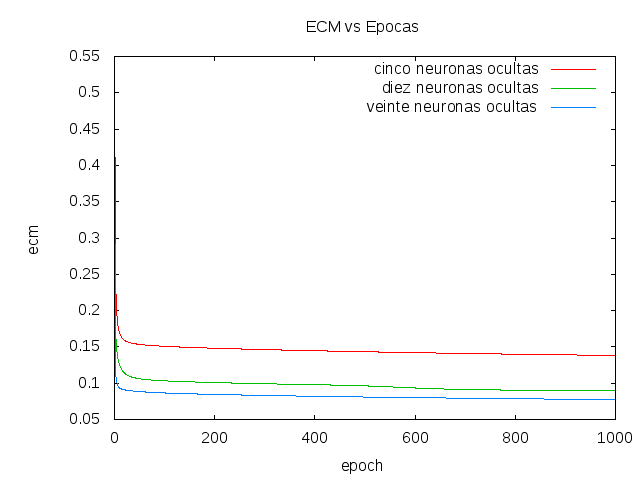
\includegraphics[width=0.7\textwidth]{recursos/ecm_pr1}
\end{figure} 

Al ser linealmente dependiente el problema, vemos que con 5, 10 y 20 neuronas, tiene resultados mas o menos igual de lisos, dado que con ese número de neuronas basta para calcular una solución, es decir, dibujar una frontera de decisión que vaya reduciendo paulatinamente el error cuadrático medio, siendo cuanto mayor el número de neuronas, mayor la eficacia de ésta frontera.

Ahora veremos el error de éste resultado:

\begin{figure}[h!]
    \label{fig:error_pr1}
  \centering
       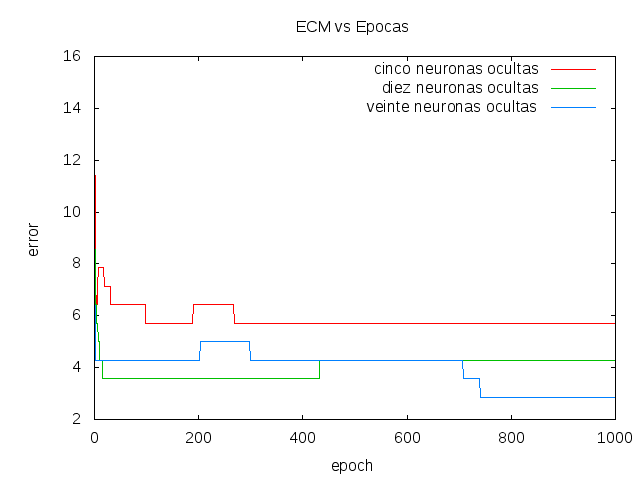
\includegraphics[width=0.7\textwidth]{recursos/error_pr1}
\end{figure} 

Podemos observar errores muy bajos, cercanos al 4\% en caso de 5 y 10 neuronas, y al 2\% en caso de 20 neuronas, suponiendo ésto una mejora de cerca del 5\% respecto al Perceptrón Simple.

En cuanto al problema real 2, dará un resultado aproximadamente (o ojo) un 10-15\% mayor, debido a que el problema de ese fichero es el ruido que tiene, y el Perceptrón permite una frontera de decisión más flexible.

Observemos ahora los resultados. Realizaremos el mismo estudio que en el problema real 1, con el mismo número de neuronas y con las mismas variables (ECM y error de training). Empezamos analizando el ECM:

\begin{figure}[h!]
    \label{fig:ecm_pr2}
  \centering
       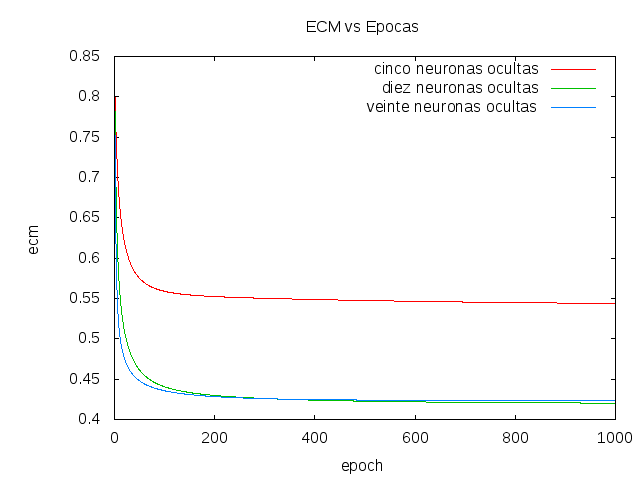
\includegraphics[width=0.7\textwidth]{recursos/ecm_pr2}
\end{figure} 

Aquí podemos ver que en caso de 5 neuronas, su comportamiento es muy inferior (mayor ECM siempre) que con 10 y 20 neuronas, siendo estos dos muy cercanos. Sin embargo, es ligeramente superior el comportamiento de la red con 10 neuronas, al de 20. Ésto es debido, a la gran cantidad de ruido (dado el gran número de patrones de entrenamiento), en el conjunto de entrenamiento, que provoca un sobreaprendizaje negativo en caso de las 20 neuronas.

Ahora observemos el error en este caso:

\begin{figure}[h!]
    \label{fig:error_pr2}
  \centering
       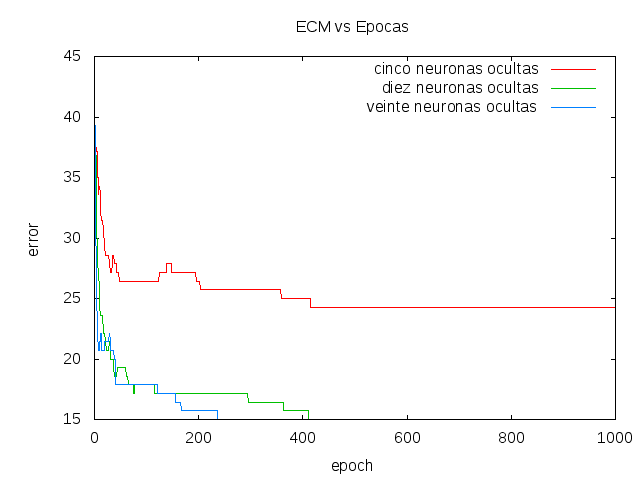
\includegraphics[width=0.7\textwidth]{recursos/error_pr2}
\end{figure} 


\newpage
% 3 Caso real
%%%%%%%%%%%%%%%%%%%%%%%%%%%%%%%%%%%%%%%%%%%%%%%%%%%%%%%%%%%%%%%%%%%%%%%%%%%
\section{Predicci\'on con ejemplos de m\'as clases}
En este ejercicio miraremos el rendimiento del Perceptrón Multicapa en un problema con más de 2 clases, en concreto, 3 (problema real 3).

En un análisis preliminar, sin ver los atributos, podemos decir que será eficaz en el caso de que tenga fronteras de decisión definidas y sin mucho ruido.

Una vez hecha la ejecución, vamos a comparar el rendimiento en aprendizaje y test, midiendo el ECM y el porcentaje de error, con 5, 10 y 20 neuronas ocultas.

La ejecución llega a convergencia en training con las 10 y 20 neuronas, siendo antes la convergencia en el caso de 10 neuronas que en el de 20.

Observemos el gráfico del ECM:

\begin{figure}[h!]
    \label{fig:ecm_pr3}
  \centering
       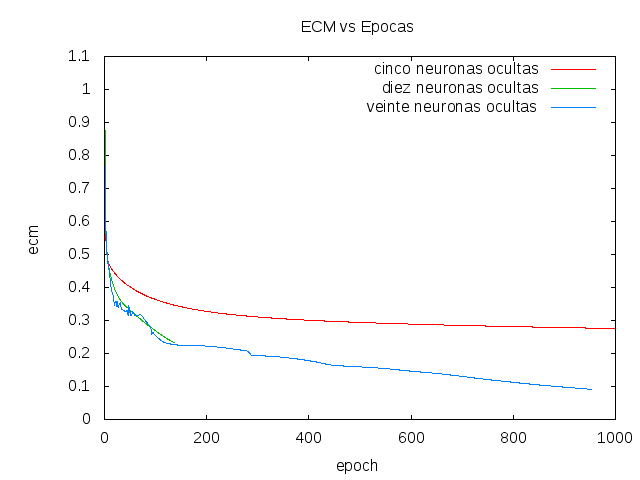
\includegraphics[width=0.7\textwidth]{recursos/ecm_pr3}
\end{figure}

Aquí podemos ver  que el ECM en caso de 5 neuronas se mantiene en reducción continua, mientras que con 10 y 20, converge. Eso puede ser debido a cierta frontera de decisión definida que son capaces de encontrar con 10 y 20 neuronas. Comentaremos sobre error de test, al comentar los errores.

Se ve que tiene una tasa irregular de reducción del ECM en el caso de 20 neuronas, al subir el número de neuronas, sube el ECM en ocasiones, debido probablemente en problemas de fronteras de decisión demasiado complejas.

Ahora observemos el error de entrenamiento:

\begin{figure}[h!]
    \label{fig:error_pr3}
  \centering
       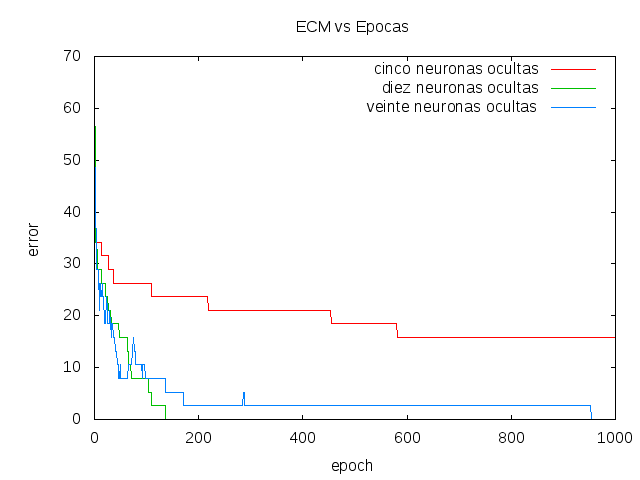
\includegraphics[width=0.7\textwidth]{recursos/error_pr3}
\end{figure} 

Aquí podemos observar que, efectivamente, llega a 0 de error en el caso de 10 y 20 neuronas, una por la época 130, y otro por la época 900, respectivamente.

Si comparamos la gráfica de error medio de 20 y y de ECM, podemos ver una coincidencia a la subida del ECM con la subida del error, debido a, como se comentó con anterioridad, la frontera de decisión transitoria peor, que luego se corrige sola.

\newpage
% 4 - Datos grandes
%%%%%%%%%%%%%%%%%%%%%%%%%%%%%%%%%%%%%%%%%%%%%%%%%%%%%%%%%%%%%%%%%%%%%%%%%%%
\section{Predicción sobre problemas complejos}

Ahora tendremos que intentar clasificar con el Perceptrón Multicapa un archivo con diferencia muy grande en sus atributos de entrada. Evaluaremos así la eficacia de este tipo de redes ante entradas con diferencias notables de peso.

En teoría, el Perceptrón Multicapa es muy sensible ante estas cosas, dado que el valor que llegue condiciona mucho la funcion lambda que realizará, provocando cierta dominancia.

Las estadísticas que realizamos sobre los datos son los siguientes:
\begin{figure}[!ht]
\centering
   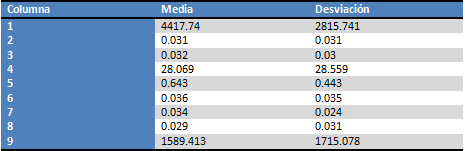
\includegraphics[width=\textwidth]{recursos/tabla}
            \caption{Tabla estadística de datos}
            \label{fig:stat_pr4}
\end{figure}
\newpage
% 5 - Normalización
%%%%%%%%%%%%%%%%%%%%%%%%%%%%%%%%%%%%%%%%%%%%%%%%%%%%%%%%%%%%%%%%%%%%%%%%%%%
\section{Optimizando el algoritmo para problemas complejos - Normalizaci\'on}

Como pudo apreciarse en la sección anterior, el aprendizaje no alcanzó un nivel tan bueno como el esperado, además de oscilar de manera increible época a época. La explicación más precisa de esto se debe a la varianza y la disperción de los datos, lo que ocasiona que se trabajen con valores, en módulo, muy grandes y chicos a la vez. Dada la estructura del algoritmo de Backpropagation (descenso por el gradiente), los patrones de entrenamiento los cuales tengan valores más grandes lograran imponerse sobre los más chicos, teniendo un efecto mucho más importante, lo cual debería ser irrelevante a la hora de clasificar estos patrones. Por otra parte, si bien no ocurre aquí, al trabajar con valores tan grandes y tan chicos a la vez, los algoritmos son menos robutos, numéricamente, y causan una convergencia más lenta. Una explicación detallada del asunto puede encontrarse en [Y. LeCunn, L.Bottou, G.B.Orr, K.R.Muller, “Eficient BackProp” Lecture Notes In Computer Science, vol. 1524, Springer-Verlag, London, pp. 8-10, 1998.]


\begin{figure}[!ht]
\centering
    \begin{subfigure}[b]{0.5\textwidth}            
            \centering
            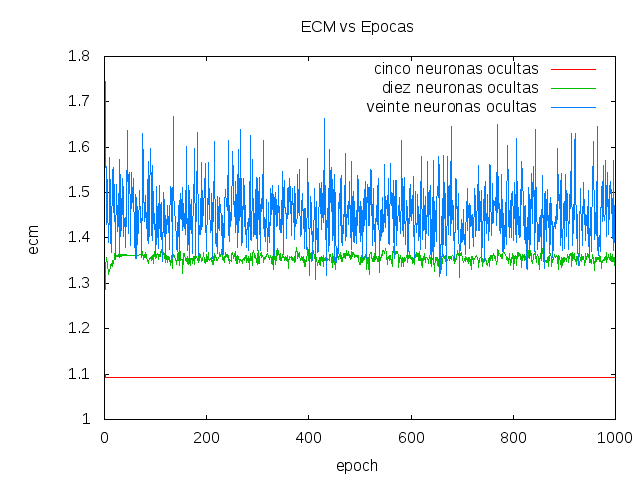
\includegraphics[width=\textwidth]{recursos/ecm_pr4}
            \caption{Datos no normalizados}
            \label{fig:ecm_pr4}
    \end{subfigure}%
     %add desired spacing between images, e. g. ~, \quad, \qquad etc.
      %(or a blank line to force the subfigure onto a new line)
    \begin{subfigure}[b]{0.5\textwidth}
            \centering
            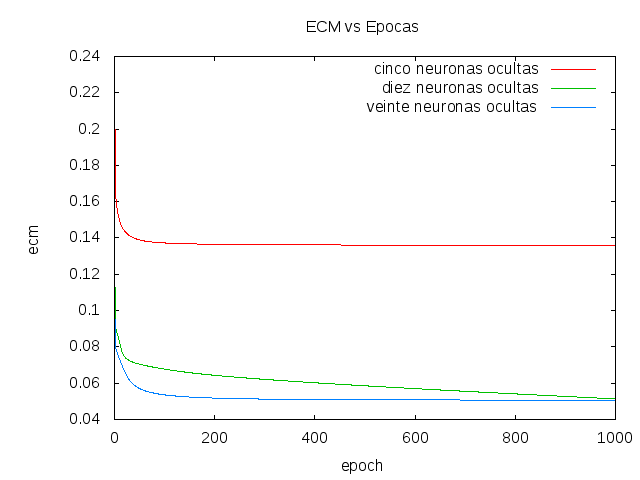
\includegraphics[width=\textwidth]{recursos/ecm_pr4_norm}
            \caption{Datos normalizados}
            \label{fig:ecm_pr4_norm}
    \end{subfigure}
    \caption{Evoluci\'on del ECM en las distintas \'epocas}
  \label{fig:ecm_vsnorm}
\end{figure}

%Grafico de ECM

Particularmente, en los gráficos podemos apreciar que mientras el algoritmo sin normalizar no converge para algunos casos (por ejemplo, con 20 neuronas en la capa oculta queda oscilando entre un ECM de 1,3 y 1,7), en el caso normalizado el algoritmo converge a valores mucho menores (del orden de las 20 veces menor) en una cantidad de iteraciones entre las 50 y las 100 según el caso.


\begin{figure}[!ht]
\centering
    \begin{subfigure}[b]{0.5\textwidth}            
            \centering
            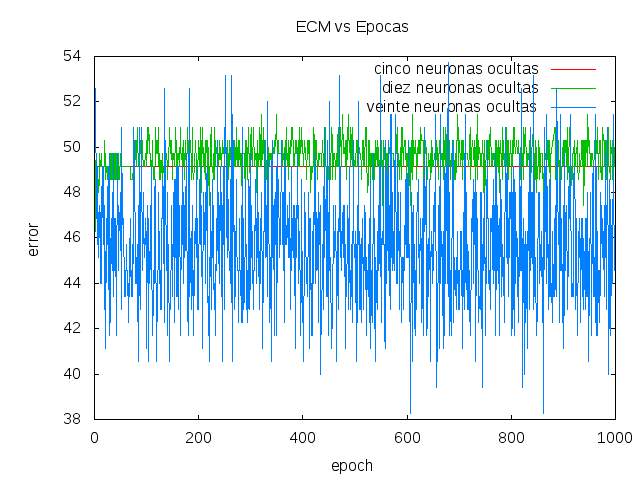
\includegraphics[width=\textwidth]{recursos/error_pr4}
            \caption{Datos no normalizados}
            \label{fig:error_pr4}
    \end{subfigure}%
     %add desired spacing between images, e. g. ~, \quad, \qquad etc.
      %(or a blank line to force the subfigure onto a new line)
    \begin{subfigure}[b]{0.5\textwidth}
            \centering
            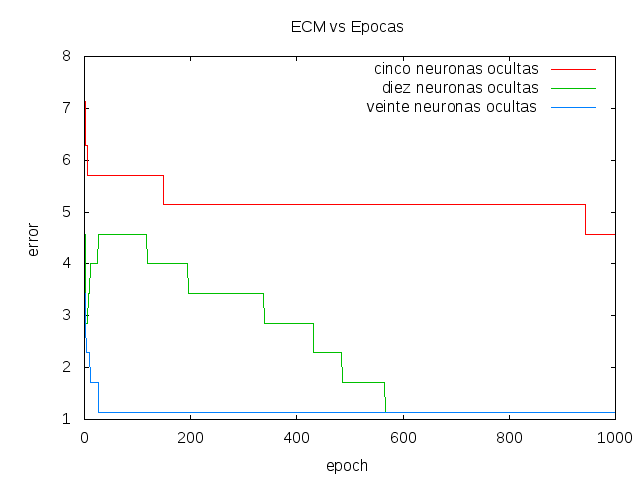
\includegraphics[width=\textwidth]{recursos/error_pr4_norm}
            \caption{Datos normalizados}
            \label{fig:error_pr4_norm}
    \end{subfigure}
    \caption{Evoluci\'on del porcentaje de error en training}
  \label{fig:error_vsnorm}
\end{figure}

%Grafico de Error

Por otra parte, podemos notar como el porcentaje de error en training se estabiliza, alcanzando valores cercanos al 5\%, mientras en los otros casos conseguiamos oscilaciones entre los 50\% y los 30\%. La conclusión de este procedimiento es obvia, normalizar los valores pueden transformar una red inservible (dado que predice con precisión de 40\% aproximadamente) a una red precisa, con un margen de 5\% de error.

\newpage


% 6 - Prediccion
%%%%%%%%%%%%%%%%%%%%%%%%%%%%%%%%%%%%%%%%%%%%%%%%%%%%%%%%%%%%%%%%%%%%%%%%%%%
\section{Predicciones sobre datos no etiquetados}
Aquí vamos a realizar la clasificación de un fichero de datos desconocido. Para ello, realizaremos un entrenamiento con el 100\% de los elementos del problema real 2, y luego ejecutaremos el algoritmo de clasificación sobre el fichero de clases desconocidas, obteniendo el fichero de salida que nos piden.

\newpage

% Conclusiones
%%%%%%%%%%%%%%%%%%%%%%%%%%%%%%%%%%%%%%%%%%%%%%%%%%%%%%%%%%%%%%%%%%%%%%%%%%%
\section*{Conclusiones}
\addcontentsline{toc}{section}{Conclusiones}
A lo largo de este trabajo topamos con las distintas virtudes de esta técnica de aprendizaje. Por un lado, en la primera parte, pudimos apreciar como un Perceptrón Multicapa puede resolver problemas que las demás técnicas de aprendizaje que aprendimos podían (NAND, NOR) y algunos que estas no (XOR). Esto nos permitió concluir que el poder de este autómata para predecir\/aprender es mayor a los aprendidos antes, algo que vimos de manera teórica en clase, pero pudimos comprobar empíricamente.

Por otra parte, pudimos apreciar el poder de esta técnica para enfrentarse a problemas de otra magnitud, donde la clasificación se hace con más datos y se tiene una cantidad mayor de categorías que dos (a lo que estabamos acostumbrados). Si bien, al contrario de lo que esperabamos, el Perceptrón encontró algunos problemas para afrontar tipos de datos con varianzas altas, al aplicar la normalización estos problemas desaparecieron. Esto nos permite concluir algo fundamental, el Perceptrón tiene un poder para aprender inmenso. Los distintos problemas que pueda enfrentar no son esenciales de la técnica, sino que pueden ser corregidos con cambios pequeños, como en este caso la Normalización.

Este trabajo nos enseñó que tenemos que debemos considerar a los Perceptrones Multicapa cada vez que queramos hacer una clasificación. Si bien pude parecer que no funciona, un análisis más preciso puede corregir fácilmente esas dificultades. En pocas palabras: ``Que vivan los Perceptrones''.




\end{document}
